
\section{块状链表}

\href{./images/kuaizhuanglianbiao.png "./images/kuaizhuanglianbiao.png"}{\begin{figure}[h]
\centering
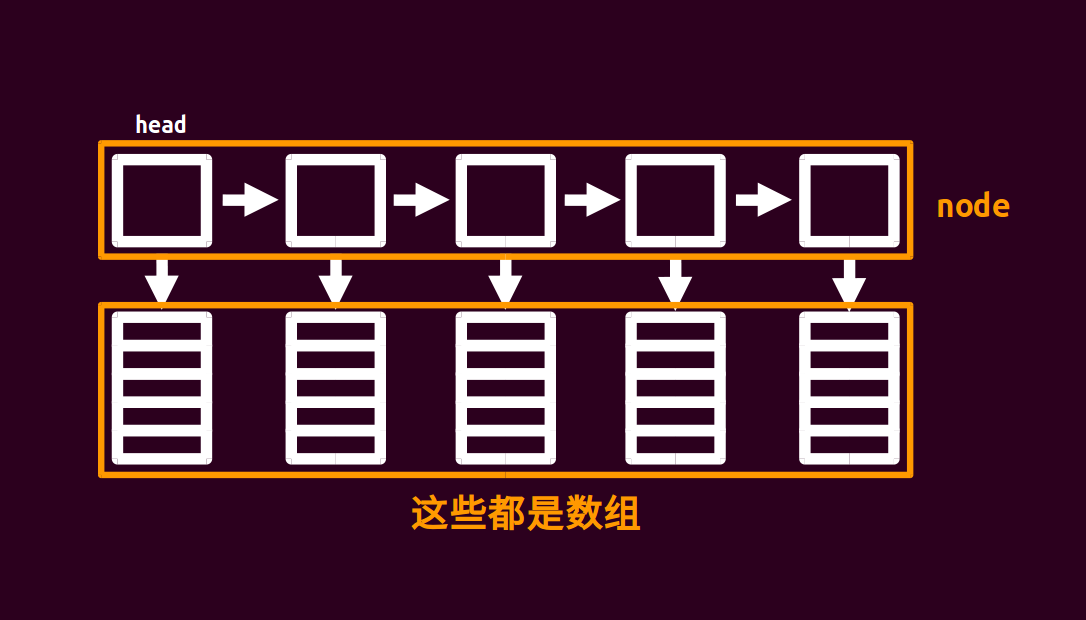
\includegraphics[width=0.5\textwidth]{images/kuaizhuanglianbiao.png} 
\caption{./images/kuaizhuanglianbiao.png}
\end{figure}}

大概就长这样……

不难发现块状链表就是一个链表,每个节点指向一个数组。

我们把原来长度为 n 的数组分为 $\sqrt{n}$ 个节点,每个节点对应的数组大小为 $\sqrt{n}$ 。

所以我们这么定义结构体,代码见下。

其中 \texttt{sqn} 表示 \texttt{sqrt(n)} 即 $\sqrt{n}$,\texttt{pb} 表示 \texttt{push_back},即在这个 \texttt{node} 中加入一个元素。

\begin{cppcode}
struct node {
  node* nxt;
  int size;
  char d[(sqn << 1) + 5];
  node() { size = 0, nxt = NULL, memset(d, 0, sizeof(d)); }
  void pb(char c) { d[size++] = c; }
};
\end{cppcode}

块状链表应该至少支持:分裂、插入、查找。

什么是分裂?分裂就是分裂一个 \texttt{node},变成两个小的 \texttt{node},以保证每个 \texttt{node} 的大小都接近 $\sqrt{n}$ (否则可能退化成普通数组)。当一个 \texttt{node} 的大小超过 $2\times \sqrt{n}$ 时执行分裂操作。

分裂操作怎么做呢?先新建一个节点,再把被分裂的节点的后 $\sqrt{n}$ 个值 \texttt{copy} 到新节点,然后把被分裂的节点的后 $\sqrt{n}$ 个值删掉(\texttt{size--}),最后把新节点插入到被分裂节点的后面即可。

块状链表的所有操作的复杂度都是 $\sqrt{n}$ 的。

还有一个要说的。

随着元素的插入(或删除),$n$ 会变, $\sqrt{n}$ 也会变。这样块的大小就会变化,我们难道还要每次维护块的大小?

其实不然,把 $\sqrt{n}$ 设置为一个定值即可。比如题目给的范围是 $10^6$,那么 $\sqrt{n}$ 就设置为大小为 $10^3$ 的常量,不用更改它。

\begin{cppcode}
list<vector<char> > orz_list;
\end{cppcode}

\subsection{例题}

Big String POJ - 2887

题解:

很简单的模板题。代码如下:

\begin{cppcode}
#include <cctype>
#include <cstdio>
#include <cstring>
using namespace std;
static const int sqn = 1e3;
struct node {
  node* nxt;
  int size;
  char d[(sqn << 1) + 5];
  node() { size = 0, nxt = NULL; }
  void pb(char c) { d[size++] = c; }
}* head = NULL;
char inits[(int)1e6 + 5];
int llen, q;
void readch(char& ch) {
  do
    ch = getchar();
  while (!isalpha(ch));
}
void check(node* p) {
  if (p->size >= (sqn << 1)) {
    node* q = new node;
    for (int i = sqn; i < p->size; i++) q->pb(p->d[i]);
    p->size = sqn, q->nxt = p->nxt, p->nxt = q;
  }
}
void insert(char c, int pos) {
  node* p = head;
  int tot, cnt;
  if (pos > llen++) {
    while (p->nxt != NULL) p = p->nxt;
    p->pb(c), check(p);
    return;
  }
  for (tot = head->size; p != NULL && tot < pos; p = p->nxt, tot += p->size)
    ;
  tot -= p->size, cnt = pos - tot - 1;
  for (int i = p->size - 1; i >= cnt; i--) p->d[i + 1] = p->d[i];
  p->d[cnt] = c, p->size++;
  check(p);
}
char query(int pos) {
  node* p;
  int tot, cnt;
  for (p = head, tot = head->size; p != NULL && tot < pos;
       p = p->nxt, tot += p->size)
    ;
  tot -= p->size;
  return p->d[pos - tot - 1];
}
int main() {
  scanf("%s %d", inits, &q), llen = strlen(inits);
  node* p = new node;
  head = p;
  for (int i = 0; i < llen; i++) {
    if (i % sqn == 0 && i) p->nxt = new node, p = p->nxt;
    p->pb(inits[i]);
  }
  char a;
  int k;
  while (q--) {
    readch(a);
    if (a == 'Q')
      scanf("%d", &k), printf("%c\n", query(k));
    else
      readch(a), scanf("%d", &k), insert(a, k);
  }
  return 0;
}
\end{cppcode}
